\chapter{Wave Motion}
\begin{figure}[H]
    \centering
    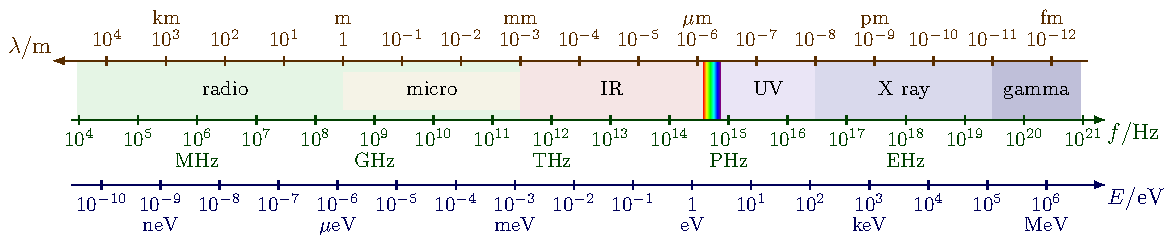
\includegraphics[width=\textwidth]{../images/em-spectrum/em-spectrum.pdf}
    \caption{\ref{source:em-spectrum} The electromagnetic spectrum.}
    \label{fig:em-spectrum}
\end{figure}
\begin{itemize}
    \item \emph{Note.} When deducing the period \(T\) of a waveform based off a graph, try to take the total time taken \(nT\) for the largest number of oscillations \(n\) possible, and then, calculate \(T=nT/n\). (Avoid directly calculating the period with \(n=1\).) This is especially important if the period is small relative to the time scale given/varies slightly with time.
    \item A \emph{progressive} wave is a wave in which \emph{energy is carried} from one point to another by means of \emph{vibrations or oscillations} within the wave. Particles within the wave are \emph{not transported along} the wave.
    \item A \emph{transverse} wave is a wave in which the direction of \emph{oscillation} of the particles (or wave
    medium) in the wave is \emph{normal} to the \emph{direction of energy transfer} of the wave.
    \item A \emph{phase} is an angle which gives a measure of the \emph{fraction of a cycle} that has been \emph{completed} by an oscillating particle or by a wave.
    \item \emph{Intensity} of a wave is the wave energy incident per unit time per unit area \emph{normal} to the wave.
    \item \emph{Polarisation} is a process where the \emph{oscillations} of the particles in a \emph{transverse wave} is restricted to a \emph{single direction}, in the plane \emph{normal} to the direction of energy transfer.
\begin{example}{}{}
    Explain why two (coherent) sources of light that are polarised in planes perpendicular to each other will not product observable interference fringes.

    \vspace{0.5\baselineskip} The displacements \(s_1\) and \(s_2\), due to each of the two waves, are in perpendicular axes. No component of \(s_1\) can ever be in the same or opposite direction as that \(s_2\). Hence, the vector sum \(s_1+s_2\) will not be able to produce distinct maxima and minima; no bright or dark fringes are formed.
\end{example}
    \item A longitudinal wave \emph{cannot be polarised} because the direction of oscillation of particles in the wave is \emph{parallel} to the direction of energy transfer in the wave.
\end{itemize}
\begin{minipage}{3cm+15.2363pt}
    \includegraphics[page=4]{../images/Malus'-Law/Malus'-Law.pdf}
\end{minipage}%
\begin{minipage}{\textwidth-3cm-15.2363pt}
    \begin{itemize}
        \item Malus' Law states that the intensity of a beam of \emph{plane polarised light} after passing through a rotatable polariser is directly proportional to the square of the cosine of the angle through which the polariser is rotated from the position that gives maximum intensity. (\(I=I_{\text{max}}\cos^2(\theta)\))
    \end{itemize}
\end{minipage}
    \begin{figure}[H]
        \centering
        \includegraphics[width=\textwidth,page=3]{../images/Malus'-Law/Malus'-Law.pdf}
        \caption{\ref{source:malus-law} An illustration of Malus' Law.}
        \label{fig:malus-law}
    \end{figure}
\begin{itemize}[label=\(\square\)]
    \item[\mbox{\FiveStarOpen}] When unpolarised light passes through a polariser, the average value of \(\cos^2(\theta)\) is \(\frac{1}{2}\) so \(I_\text{new}=\frac{1}{2}I_\text{max}\). 
    \item \begin{tabular}{|Sc|Sc|Sc|}
        \hline
        Phase Angle \(\phi\) & \(2\pi\cdot\dfrac{x}{\lambda}\) & \(2\pi\cdot\dfrac{t}{T}\)\\
        \hline
        Phase Difference \(\Delta \phi\) & \(2\pi\cdot\dfrac{\Delta x}{\lambda}\) & \(2\pi\cdot\dfrac{\Delta t}{T}\)\\
        \hline
    \end{tabular}
    \item \begin{tabular}{|Sc|Sc|Sc|Sc|}
            \hline
            \multicolumn{4}{|Sc|}{Intensity}\\
            \hline
            \multirow{2}{*}{Amplitude} & \multicolumn{3}{Sc|}{Wave}\\
            \cline{2-4}
            & Spherical & Circular & Plane\\
            \hline
            \(I \propto A^2\) & \(I \propto \dfrac{1}{r^2}\) & \(I \propto \dfrac{1}{r}\) & \begin{minipage}{3cm}
                \vspace{1mm}\begin{center}
                    \(I\) is constant\\
                \scriptsize (No spreading of waves) \normalsize
                \end{center}
            \end{minipage}\\
            \hline
        \end{tabular}
        \item When a wave travels from one medium to another, its frequency remains unchanged. The intuition: think of two ropes of different (linear) densities connected in series. It would snap if they oscillated at different frequencies.
\end{itemize}